In questa sezione si presentano le caratteristiche tensione-corrente dei dispositivi sotto analisi in questo lavoro di tesi.
In figura \ref{fig:id_vds} vengono mostrati i grafici $I_{D} - V_{DS}$ a $V_{GS}$ pari a $450mV$, mentre in figura \ref{fig:id_vgs} vengono riportati gli andamenti della caratteristica $I_D - V_{GS}$ con $V_{DS} = 450mV$.


% ! ID - VDS con VGS a 450mV
\begin{figure}[ht]
    \centering
    \adjustbox{max size={\textwidth}{\textheight}}{%
      \begin{minipage}{\textwidth}
        \centering
        % W = 100
        \includegraphics[width=0.49\textwidth]{./capitolo2/Id-Vgs_Id-Vds/NMOS/id-vds/id-vds__Vgs_450__W_100.png}
        \includegraphics[width=0.49\textwidth]{./capitolo2/Id-Vgs_Id-Vds/PMOS/id-vds/id-vds__Vgs_450__W_100.png}\\
        % W = 200
        \vspace{0.2cm}
        \includegraphics[width=0.49\textwidth]{./capitolo2/Id-Vgs_Id-Vds/NMOS/id-vds/id-vds__Vgs_450__W_200.png}
        \includegraphics[width=0.49\textwidth]{./capitolo2/Id-Vgs_Id-Vds/PMOS/id-vds/id-vds__Vgs_450__W_200.png} \\
        % W = 600
        \vspace{0.2cm}
        \includegraphics[width=0.49\textwidth]{./capitolo2/Id-Vgs_Id-Vds/NMOS/id-vds/id-vds__Vgs_450__W_600.png}
        \includegraphics[width=0.49\textwidth]{./capitolo2/Id-Vgs_Id-Vds/PMOS/id-vds/id-vds__Vgs_450__W_600.png}
      \end{minipage}
    }
  
    \caption[Caratteristica $I_D - V_{DS}$]{Caratteristica $I_D - V_{DS}$ a $V_{GS} = 450mV$ raggruppate per larghezza di canale, a sinistra MOSFET a canale N e a destra a canale P.}
    \label{fig:id_vds}
  \end{figure}



% ! ID - VGS con VDS a 450mV
\begin{figure}[ht]
    \centering
    \adjustbox{max size={\textwidth}{\textheight}}{%
      \begin{minipage}{\textwidth}
        \centering
        % W = 100
        \includegraphics[width=0.49\textwidth]{./capitolo2/Id-Vgs_Id-Vds/NMOS/id-vgs/id-vgs__Vds_450__W_100.png}
        \includegraphics[width=0.49\textwidth]{./capitolo2/Id-Vgs_Id-Vds/PMOS/id-vgs/id-vgs__Vds_450__W_100.png}\\
        % W = 200
        \vspace{0.2cm}
        \includegraphics[width=0.49\textwidth]{./capitolo2/Id-Vgs_Id-Vds/NMOS/id-vgs/id-vgs__Vds_450__W_200.png}
        \includegraphics[width=0.49\textwidth]{./capitolo2/Id-Vgs_Id-Vds/PMOS/id-vgs/id-vgs__Vds_450__W_200.png} \\
        % W = 600
        \vspace{0.2cm}
        \includegraphics[width=0.49\textwidth]{./capitolo2/Id-Vgs_Id-Vds/NMOS/id-vgs/id-vgs__Vds_450__W_600.png}
        \includegraphics[width=0.49\textwidth]{./capitolo2/Id-Vgs_Id-Vds/PMOS/id-vgs/id-vgs__Vds_450__W_600.png}
      \end{minipage}
    }
  
    \caption[Caratteristica $I_D - V_{GS}$]{Caratteristica $I_D - V_{GS}$ a $V_{DS} = 450mV$ raggruppate per larghezza di canale, a sinistra MOSFET a canale N e a destra a canale P.}
    \label{fig:id_vgs}
  \end{figure}
